\subsection{sacabench}
\label{framework:cli:sacabench}

{
\begin{wrapfigure}[16]{R}[5mm]{.5\textwidth}
    \vspace{-1.5\baselineskip}
    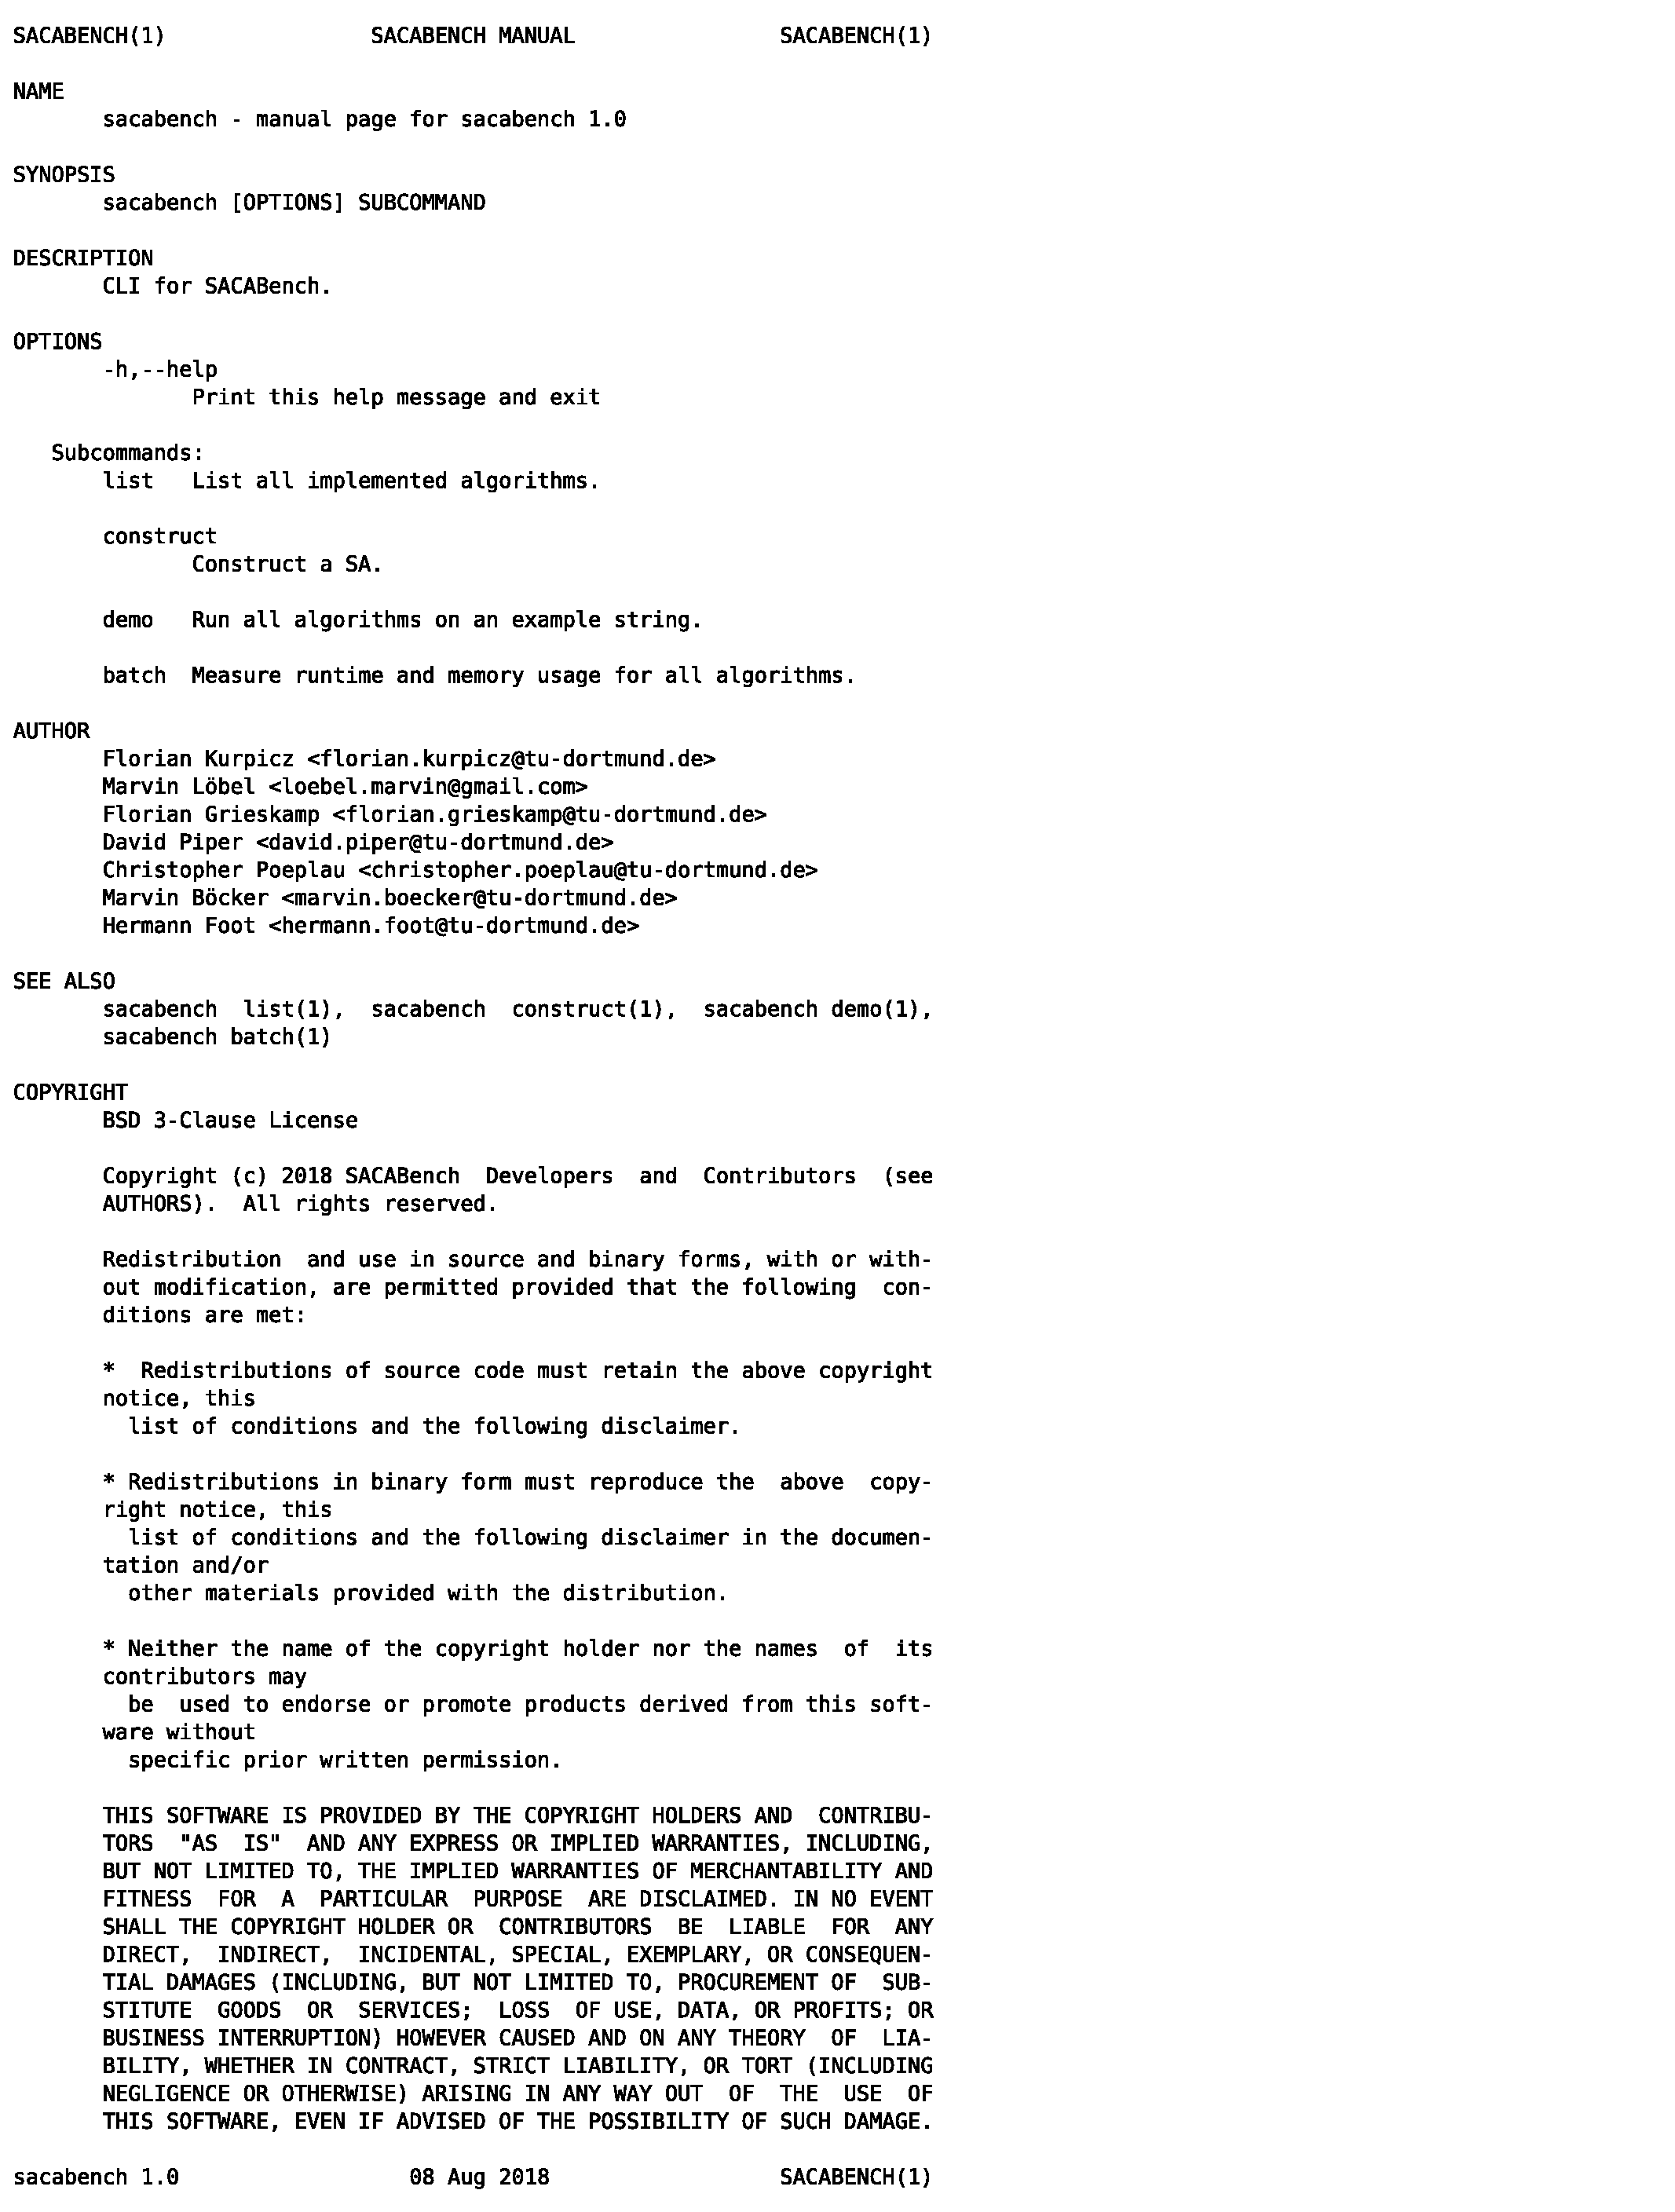
\includegraphics[page=1, viewport=0cm 32.8cm 20.5cm 47.5cm, clip, width=.5\textwidth]{{kapitel/3_framework/cli/sacabench/sacabench}.pdf}\\
    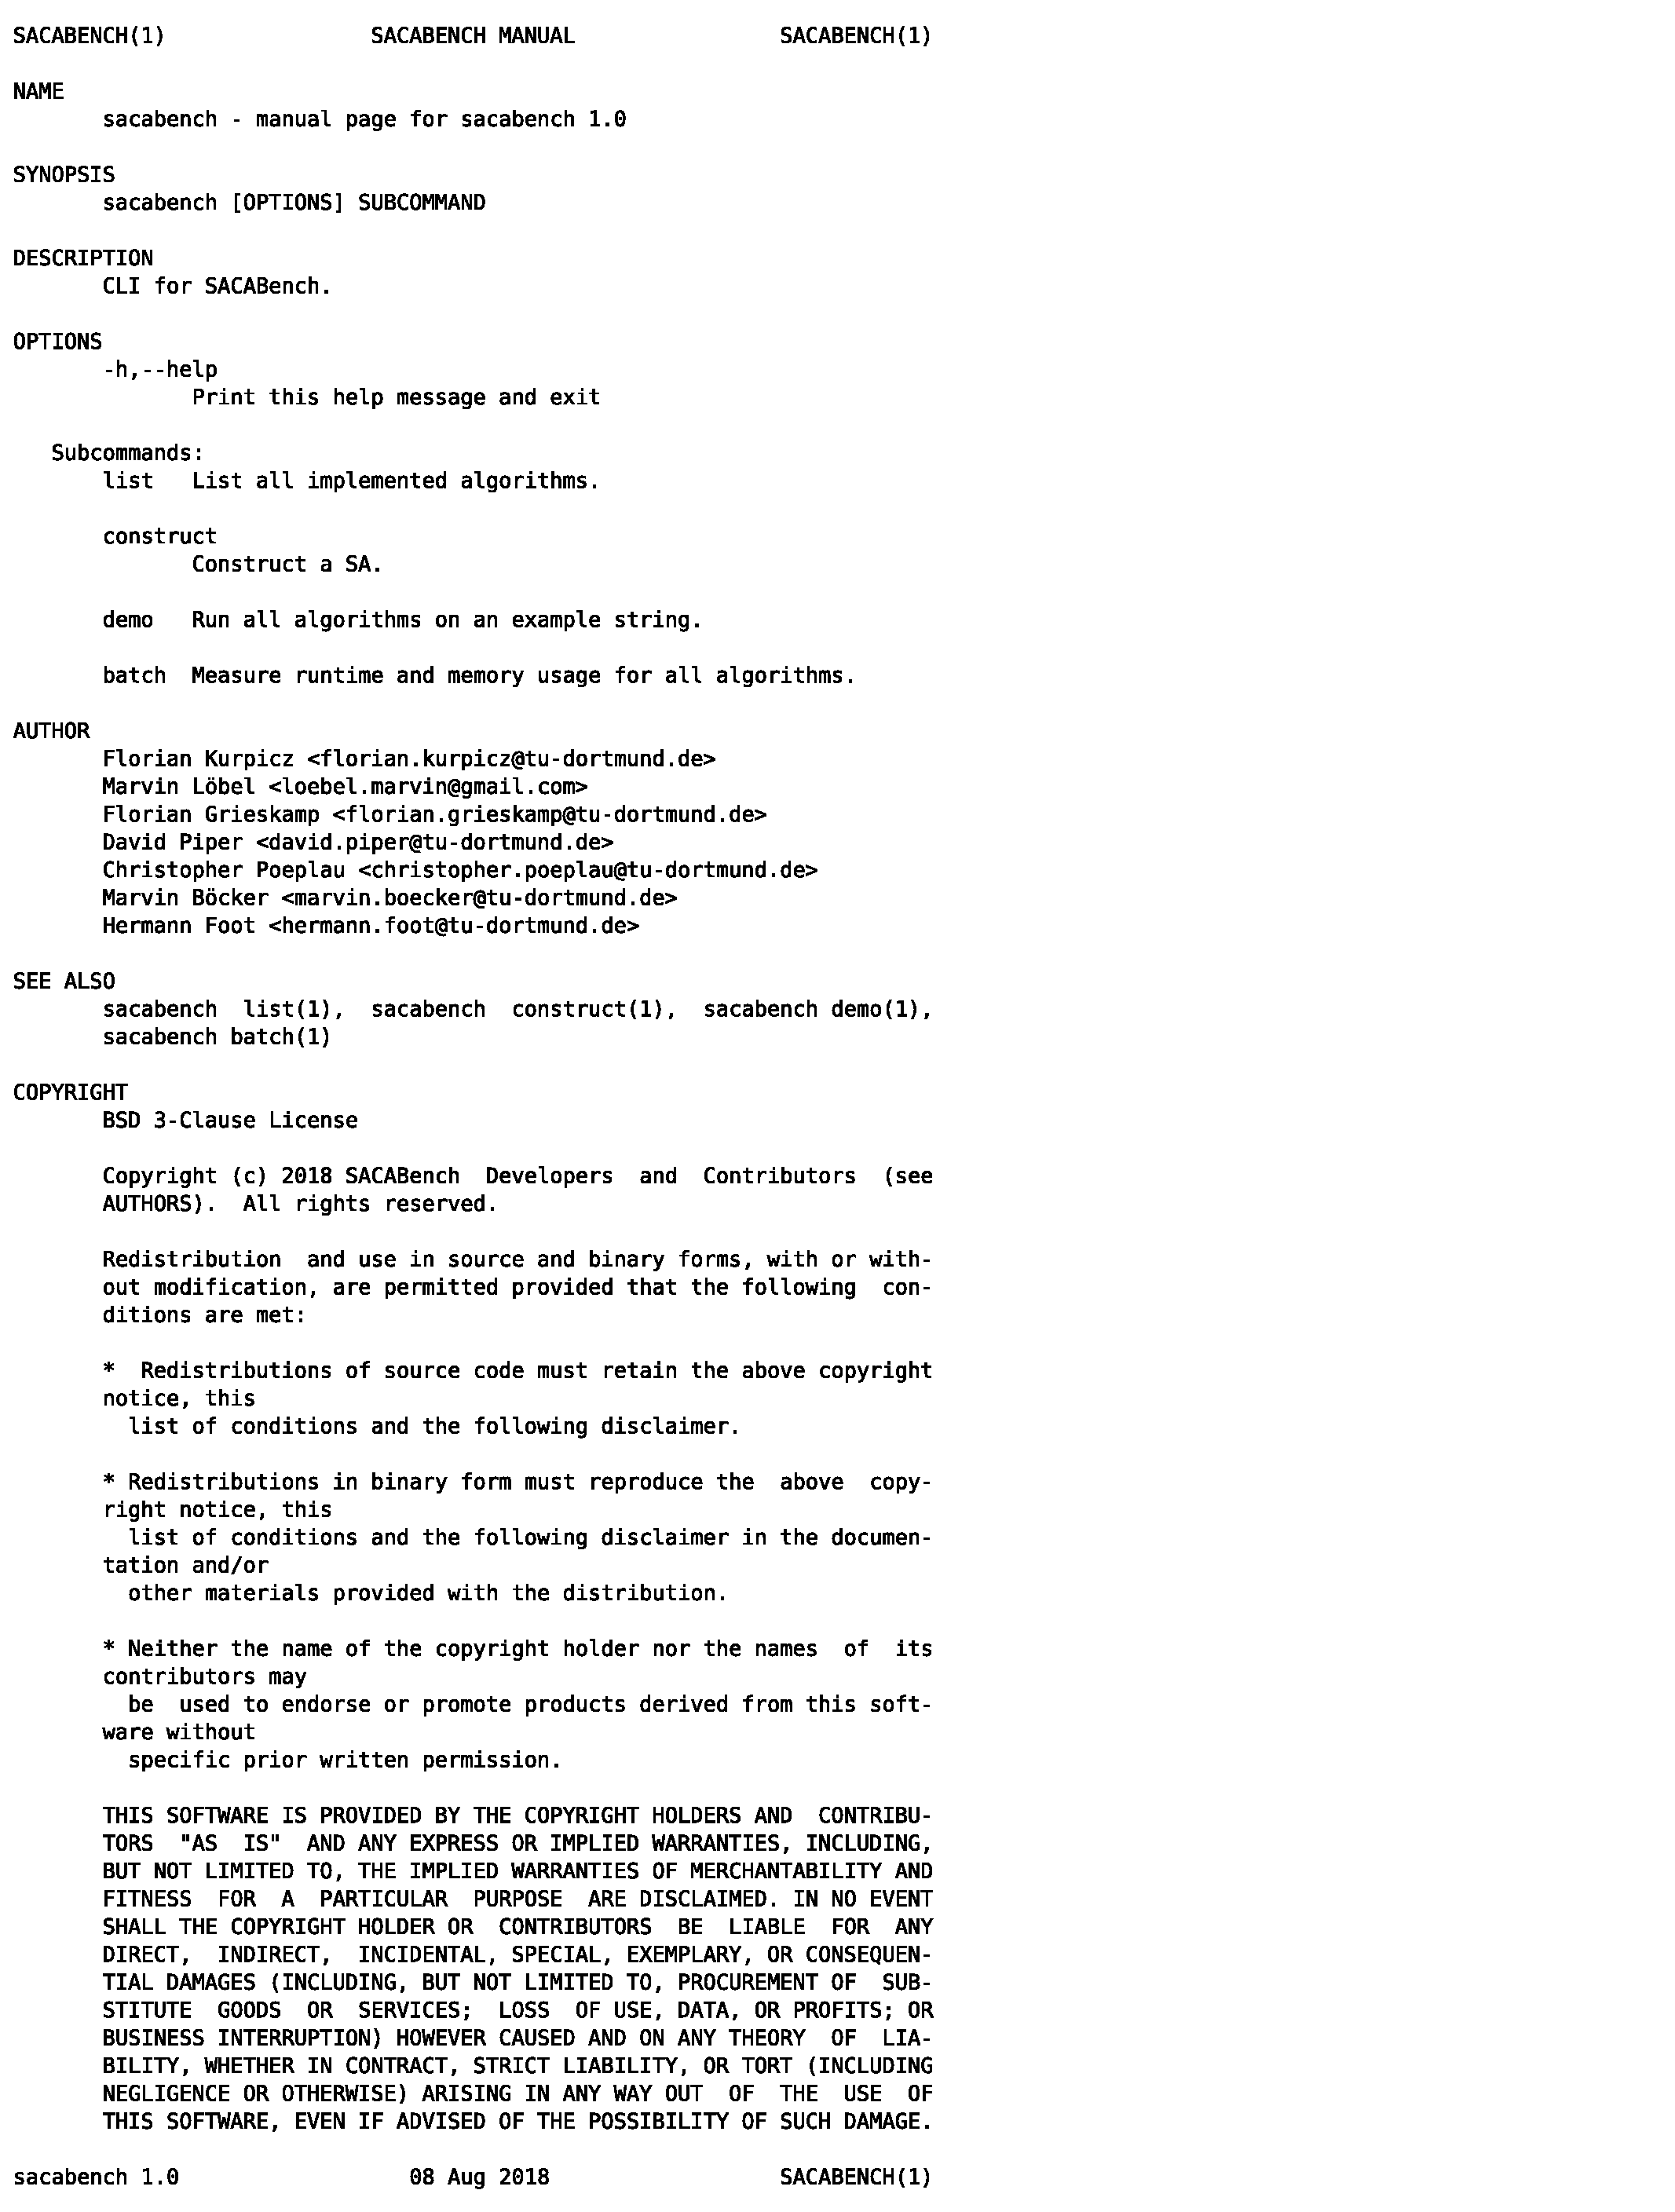
\includegraphics[page=1, viewport=0cm 25cm 20.5cm 27.3cm, clip, width=.5\textwidth]{{kapitel/3_framework/cli/sacabench/sacabench}.pdf}\\
    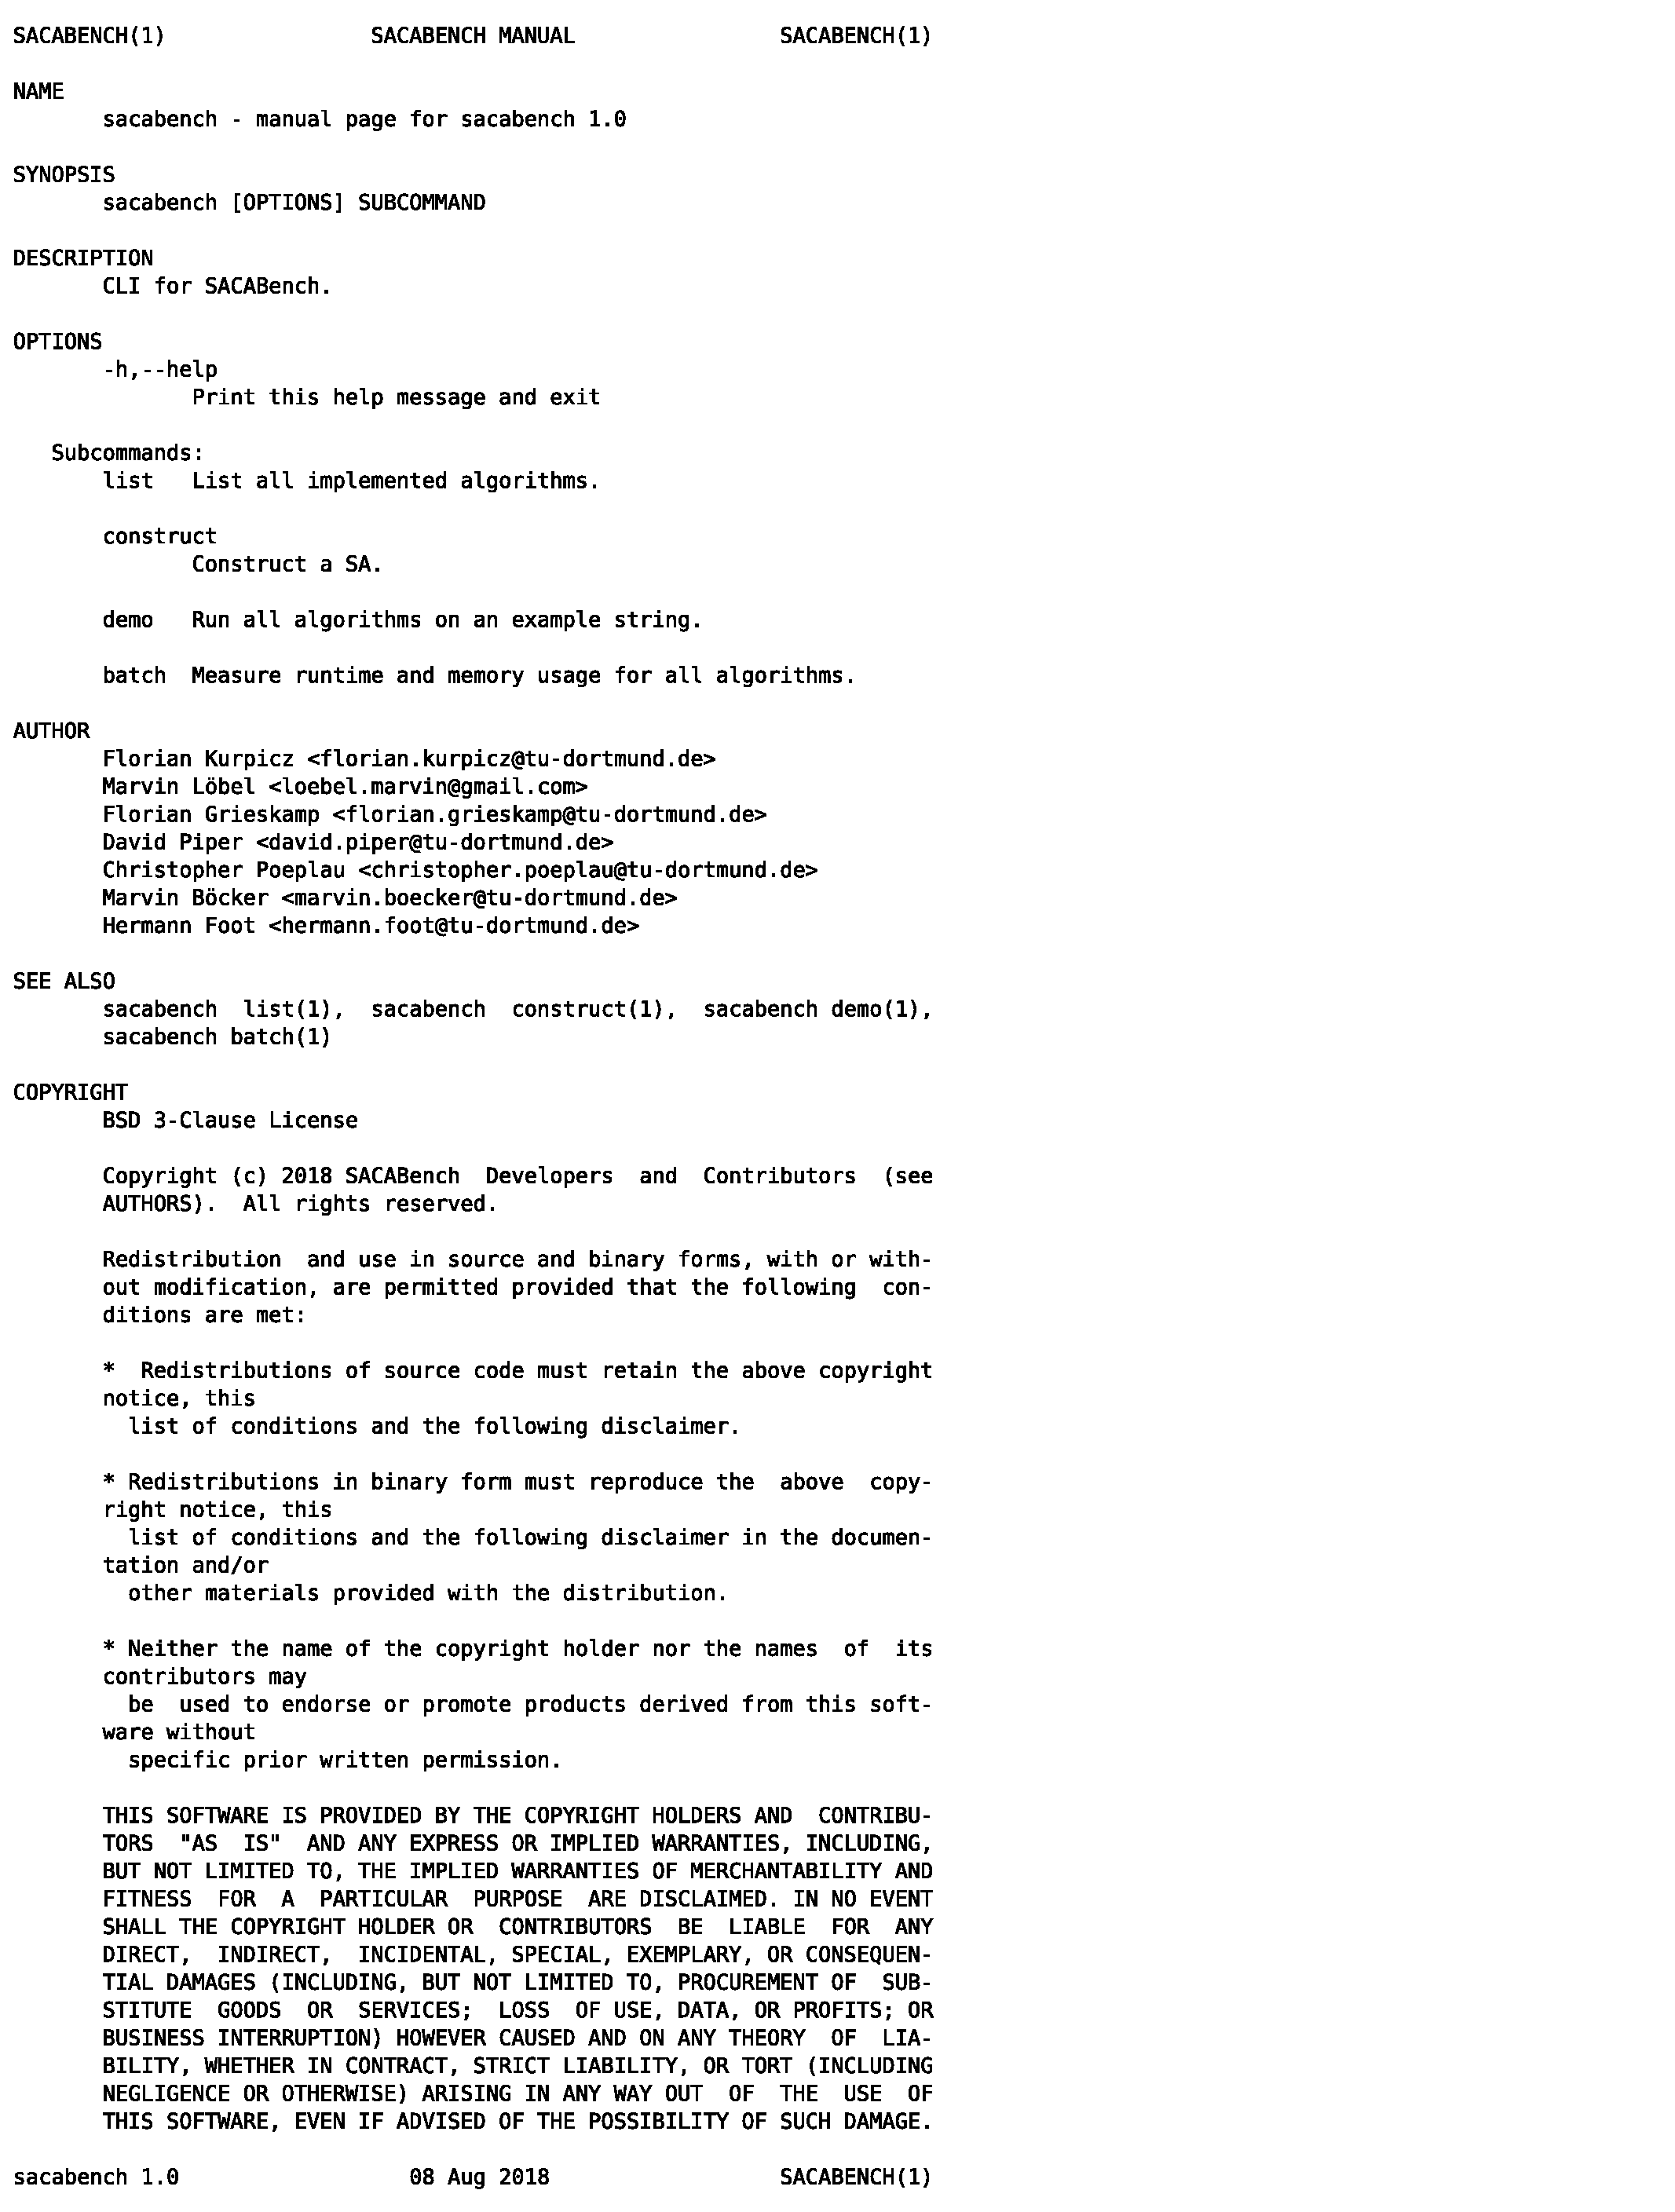
\includegraphics[page=1, viewport=0cm 0cm 20.5cm 1.5cm, clip, width=.5\textwidth]{{kapitel/3_framework/cli/sacabench/sacabench}.pdf}
    \caption{gekürzte Ausgabe von \texttt{man sacabench}}
    \label{manpage:sacabench}
\end{wrapfigure}
Das Hauptprogramm wird mit dem Befehl \texttt{sacabench} ausgeführt.
Für die einzelnen Funktionen stehen ent\-sprech\-ende Subcommands zur Verfügung.
Alle Komponenten beinhalten eine Hilfefunktion, die sich durch die Option \termfont{-h} bzw. \termfont{-{}-help} aufrufen lässt.
Die gleiche Hilfe wird außerdem ausgegeben, wenn das Programm mit ungültigen Parametern aufgerufen wird.
Für präzisere Erläuterungen der Aufrufe und Optionen stehen außerdem Man-Pages für alle Subcommands zur Verfügung.
Diese sind wie gewohnt über \termfont{man sacabench} bzw. \termfont{man sacabench [SUBCOMMAND]} aufzurufen und beinhalten neben der Beschreibung der Befehlssyntax und den Erläuterungen zur Verwendung der Optionen auch eine Liste der beteiligten Autoren, Verweise auf ähnliche Befehle und die Copyright-Bestimmungen.
Eine gekürzte Version der Man-Page für den Befehl \termfont{sacabench} ist in \cref{manpage:sacabench} zu sehen.
Alle im hier abgebildeten Man-Pages sind aus Gründen der Übersichtlichkeit um die Liste der Autoren und den Copyright-Verweis reduziert.\par
}
